The SmartSociety platform is meant to support a rather wide range of
social computation patterns (or templates). In order to provide
insight into the flexibility of the platform and the actual
interworking of components, we have developed sequence diagrams for two
'extreme' applications:
\begin{itemize}
\item AskSmartSociety! is a Q\&A service supporting hybridity. The
computational pattern here is that typical of micro-tasking
applications (\'a la Mechanical Turk, roughly speaking), where the
task in this corresponds to a question to be answered. The service
supports hybrid computation in that questions can be transparently
provided by machine peers or human peers. Quality criteria can be
specified in order to define when a chosen answer has to be presented
to the user. The scenario was used as the reference benchmark for the integration work carried out in WP8.

\item SmartShare is a ridesharing system able to account for user's
preferences and to compute recommendations based on the feedback
provided by other service users. It is what we call a 'full
negotiation' scenario, in which the computational task of finding an
agreement on the rides is left to individuals and collectives. The
platform in this case is used to carry out mainly administration tasks, in
particular keeping track of the rides and ride requests, their status
and to maintain reputation of drivers and passengers. In this setting, in particular, the OM is responsible for different kinds of synchronisation during composition, negotiation, deletions, etc. This synchronisation process plays a key role in this scenario in that it enables notifying the end users that a change has taken place. 
\end{itemize}
In the following we present details about the two aforementioned
applications. 


\subsection{Example: Ask SmartSociety}\label{sec:asksmartsoc}
\textit{Ask SmartSociety} is a simple Questions and Answer service enabled by the SmartSociety platform which has been used as the benchmark for implementing the initial version of the SmartSociety platform. It focus on tourism, which is the reference domain to be used for validating the SmartSociety vision.\\
Ask SmartSociety! will be a service where users can post questions in natural languages and peers can provide answers. Peers providing answers can represent humans (individuals or collectives) as well as machines (intelligent software agents). Peers can compose (forming collectives, hybrid or not) to provide answers. Answers can be ranked based on the reputation of the peers or on community ranking (similarly to stackoverflow). In some instances the user issuing the question can select an answer and provide feedback on the peer providing it.
Two examples (grounded in the tourism application scenarios) can help in understanding the features of the Ask SmartSociety! service:

\textit{Next week Peter will fly to Venice. He will be busy in meetings during the day but wants to explore some ‘hidden’ places at night. He could well explore various online tourist sites but he prefers to ask experts and local people. He could also google for relevant content, but he does not actually need an answer right away, he just needs to get it in one week. And having one system which allows him to query local experts, web-based recommendation services and incoming tourism institutions looks definitely appealing to him!
Alice is visiting Milano during the next week. It is his first time in Milan, and she is looking for a restaurant in the city centre. Since it is spring time, she would love eat outside and therefore  find a restaurant with a garden. Alice is also celiac, and she needs to find restaurants, which do have gluten free menus. She relies on the Ask SmartSociety! application for retrieving some suggestions on where to have dinner during her stay in Milan. She is looking for unconventional recommendations.}

Fig.~\ref{fig:dynamic_ask} illustrates how SmartSociety dynamic view is instantiated in the case of the \textit{AskSmartSociety!} application.

\begin{sidewaysfigure}
%\begin{figure}[!hbt]
\centering
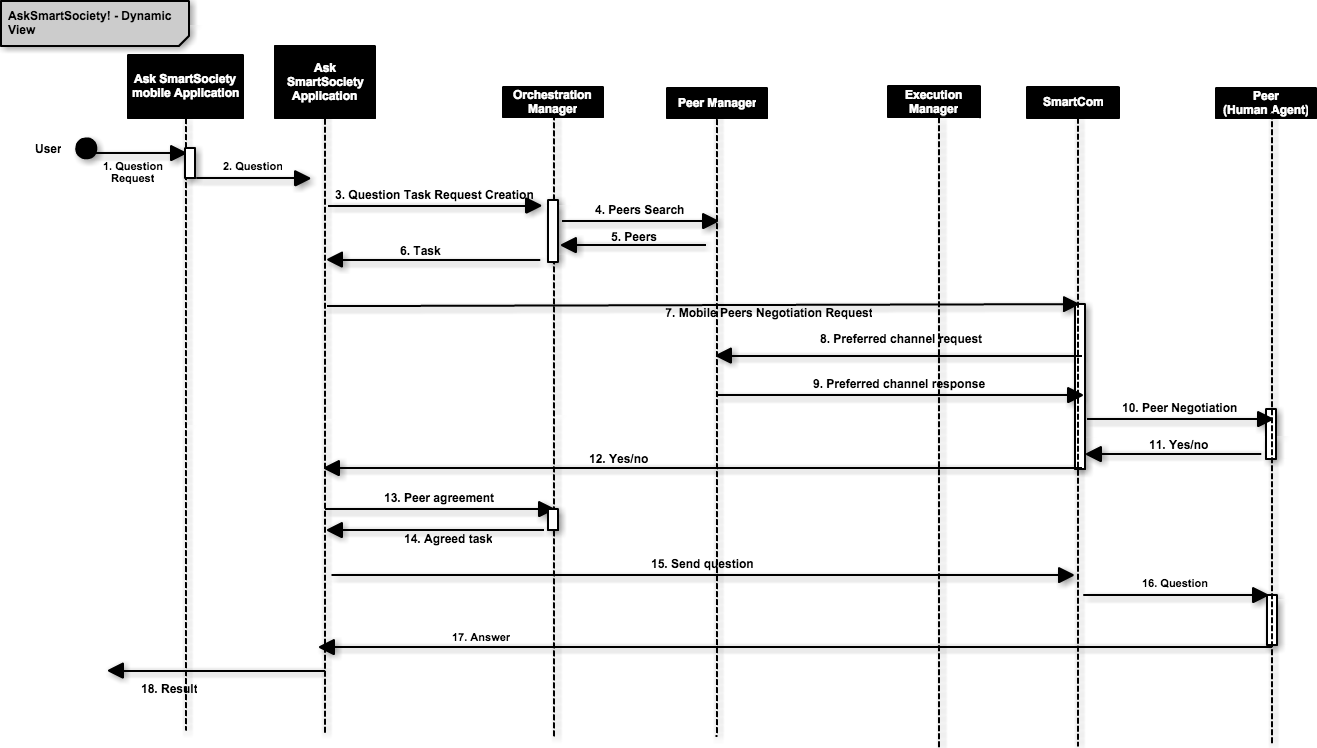
\includegraphics[width=0.9\textwidth]{./figs/sequenceAsk}%ask/ask_dynamic}
\caption{Sequence diagram for \textit{AskSmartSociety!}}
\label{fig:dynamic_ask}
\end{sidewaysfigure}

Compared to the overall sequence diagram of Fig.~\ref{fig:dynamic_view}, this is a rather simplified use case where the user application consists of a mobile application through which users can post question. The question is dispatched to the corresponding application hosted in the runtime. Such application transforms the question into a computational task to be executed by peers. Such computational task is handled by the Orchestration Manager, which identifies the most suitable composition for completing the task by querying the Peer Manager. As an example, if the question regards restaurants, the Orchestration Manager might decide to use machine peers such as, e.g., TripAdvisor or Yelp, in combination with some \textit{local knowledge} provided by human peers living in the region where the request was created. Once the composition has been created, the application recruits the peers for the execution of the task. This could potentially involve the use of incentives in order to motivate peers participation.\\
After peers have been signed up for the given task, the task execution starts. In this case, the question is sent to the peer over the preferred communication channel. In the case of machine peer, this corresponds to the proper API endpoint, whereas in the case of human peers it could be a mobile application. In the implemented scenario, we used a Twitter peer which used a hashtag to collect recommendations and a mobile application, through which users could receive questions and provide answers. In the current implementation, the Execution Manager functionality is embedded in the application itself, which interacts directly with peers exploiting the SmartCom functionalities.\\
Once the task is completed, and the answers are collected, the outcome of the computation is delivered to the users originally posting the question.

AskSmartSociety! has been prototyped to be used as both a driver of the integration process as well as to demonstrate the ability of the platform to support hybridity. Indeed, in the current prototype questions can be seamlessly answered by machine peers (in particular using the Google Search functionality) as well as human peers (using a purposeful developed mobile application). Further, a Twitter peer was developed; this is formally a machine peer, which is used to further distribute the task (in the form of the original question) to human peers, aggregating answers and feeding them back to the application. In Fig.~\ref{fig:askpeer} we display the user interface implemented in the mobile app used for testing and demonstration purposes. 
% the UX design that has been conducted for the mobile application.


\begin{figure}[!bht]
    \subfloat[Question form\label{subfig-1:dummy}]{%
      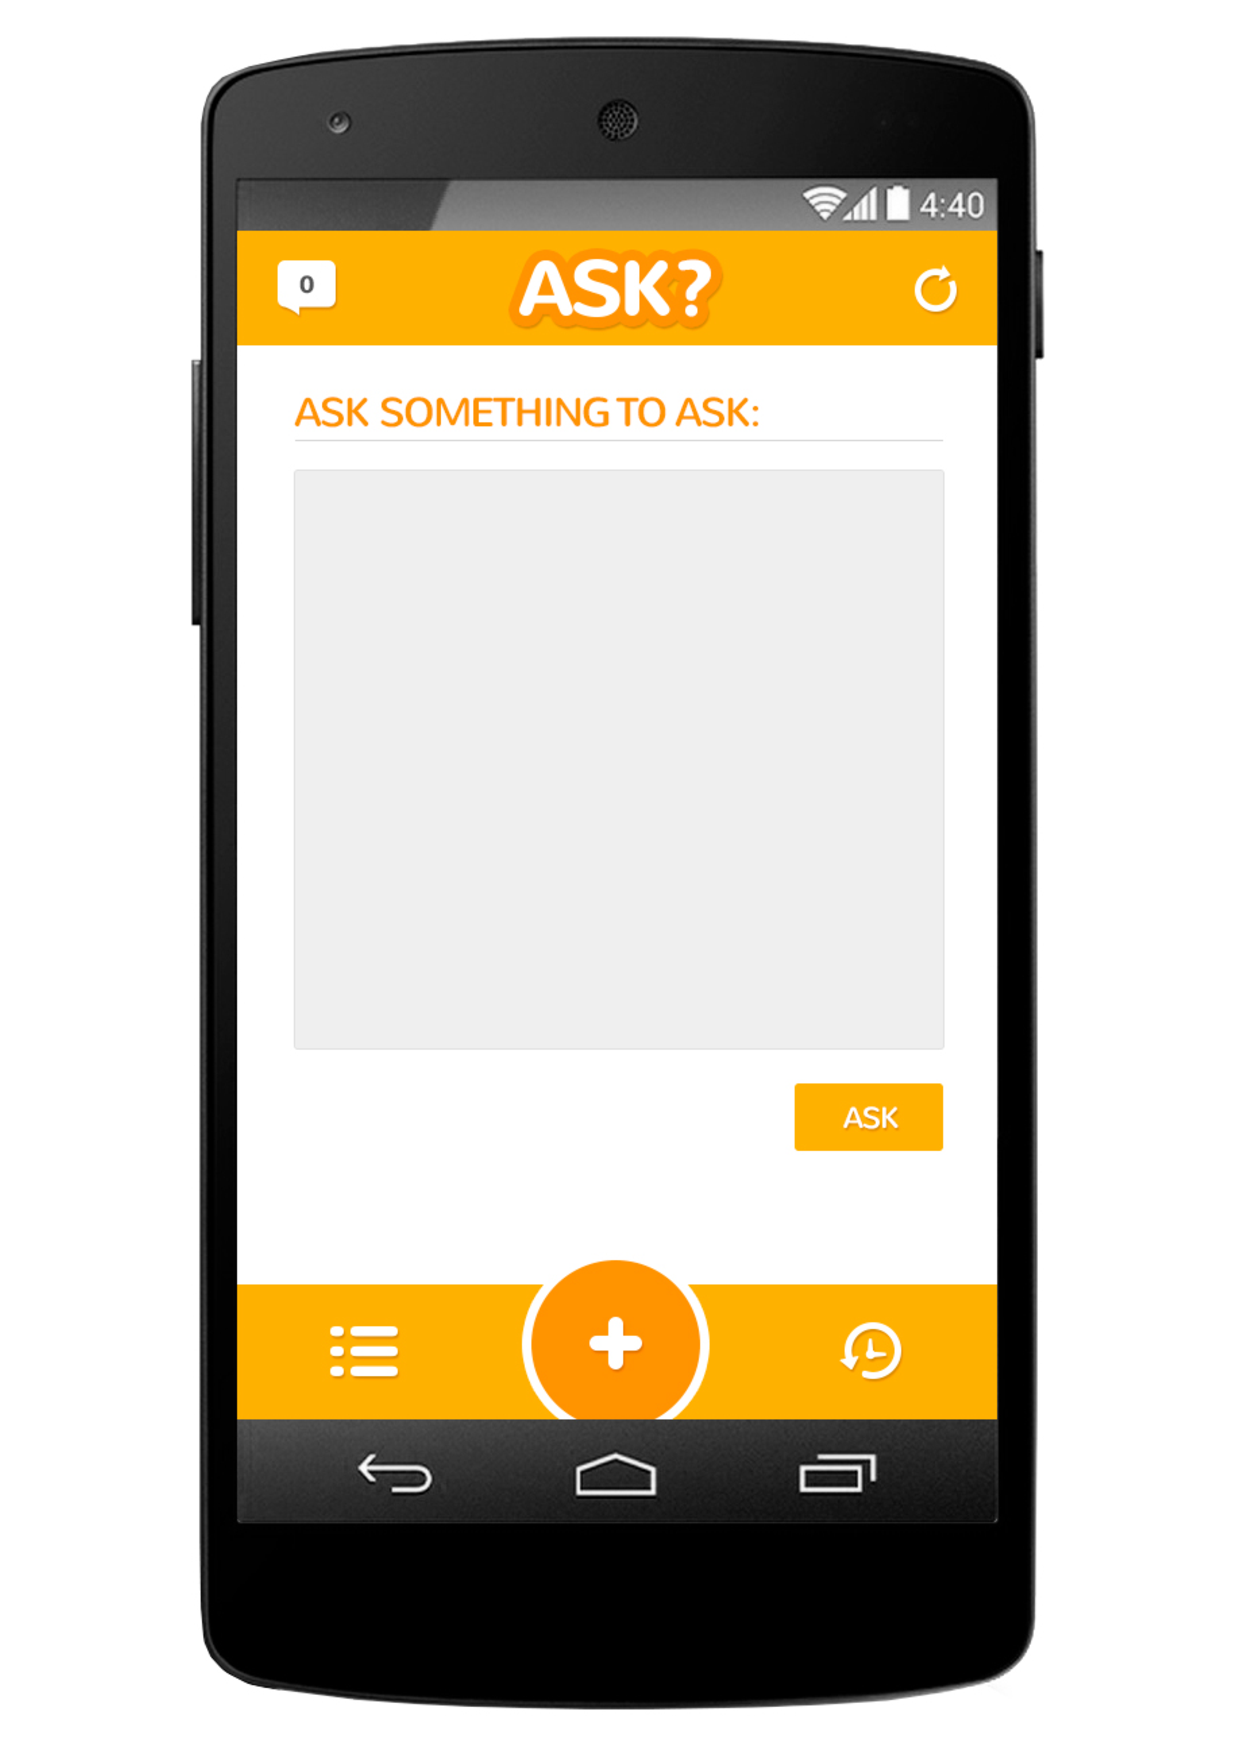
\includegraphics[width=0.2\textwidth]{./figs/ask/ask0.pdf}
    }
    \hfill
    \subfloat[Questions list\label{subfig-2:dummy}]{%
      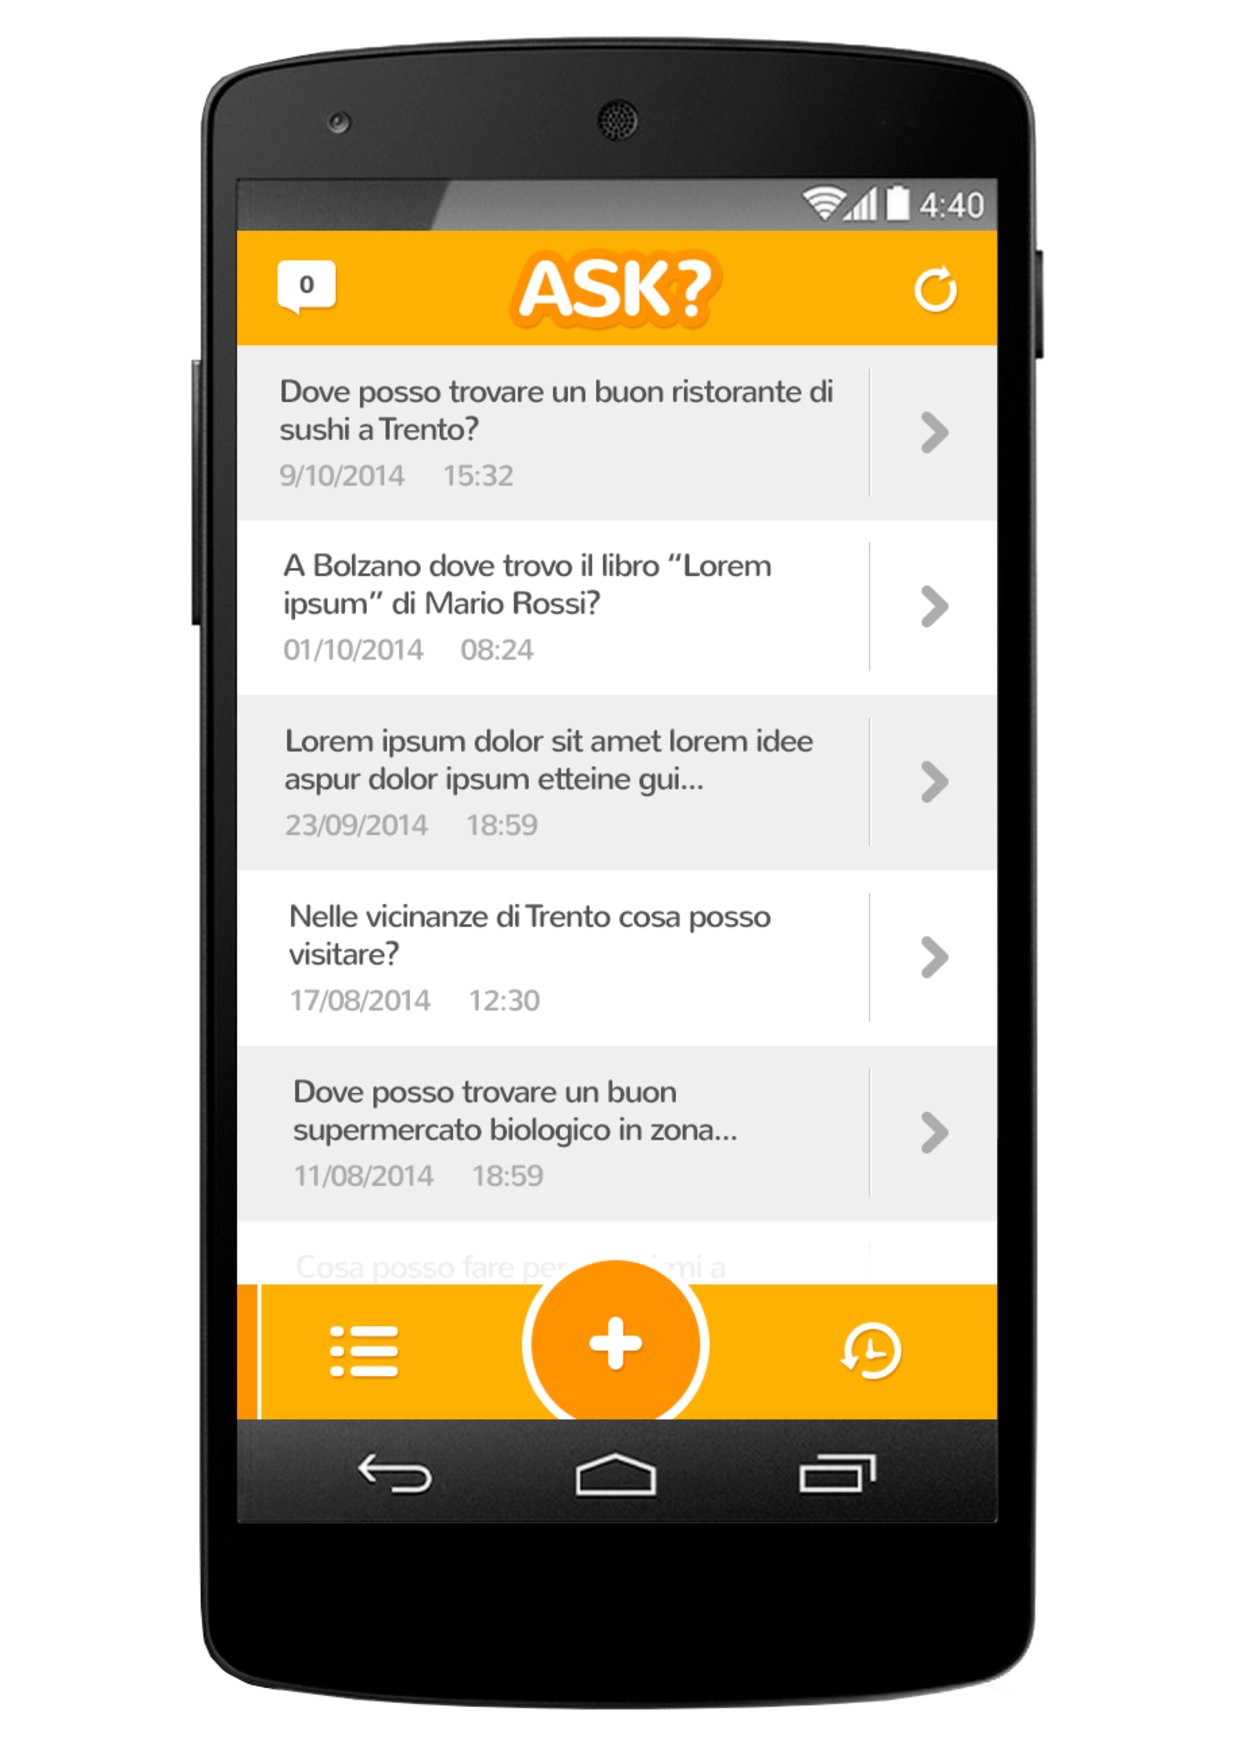
\includegraphics[width=0.2\textwidth]{./figs/ask/ask1.pdf}
    }
	\subfloat[Question\label{subfig-3:dummy}]{%
      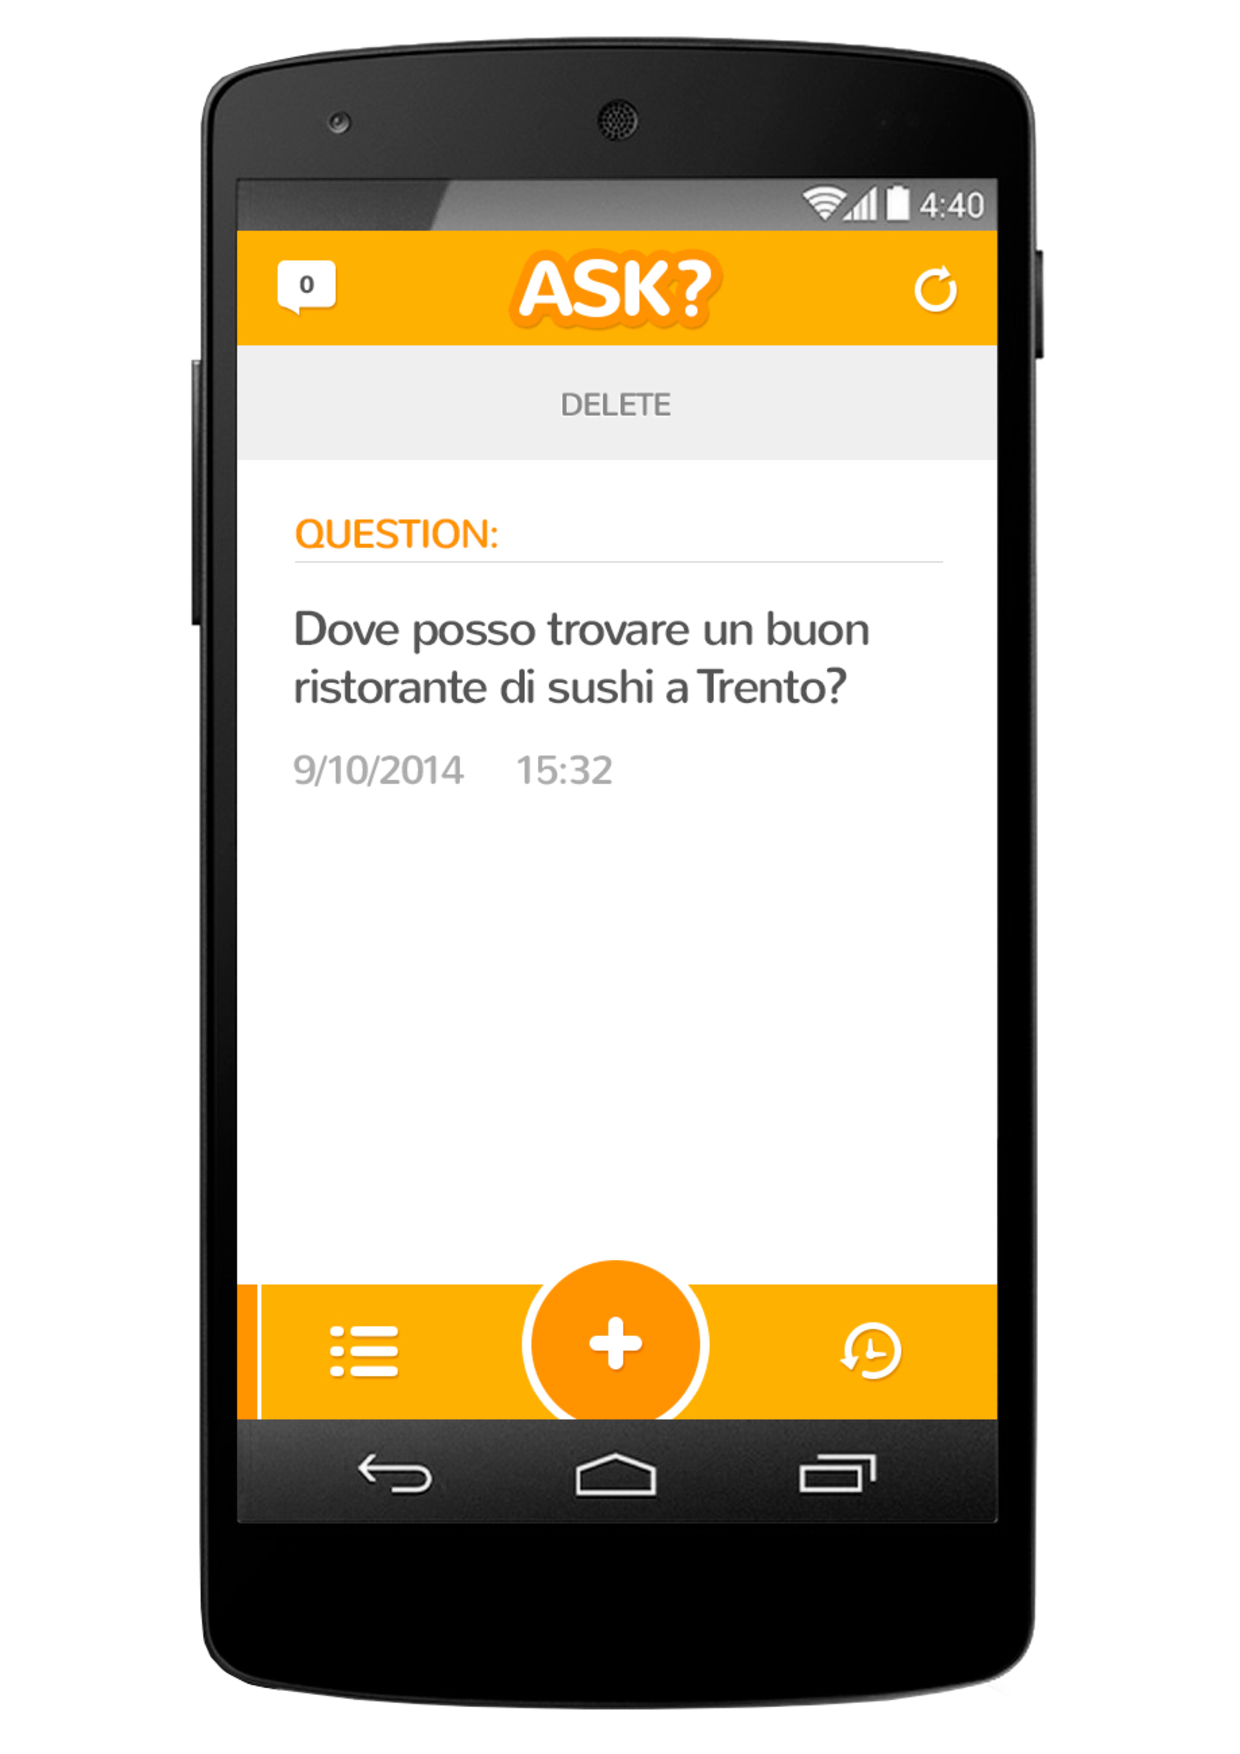
\includegraphics[width=0.2\textwidth]{./figs/ask/ask2.pdf}
    }
    	\subfloat[Question status\label{subfig-4:dummy}]{%
      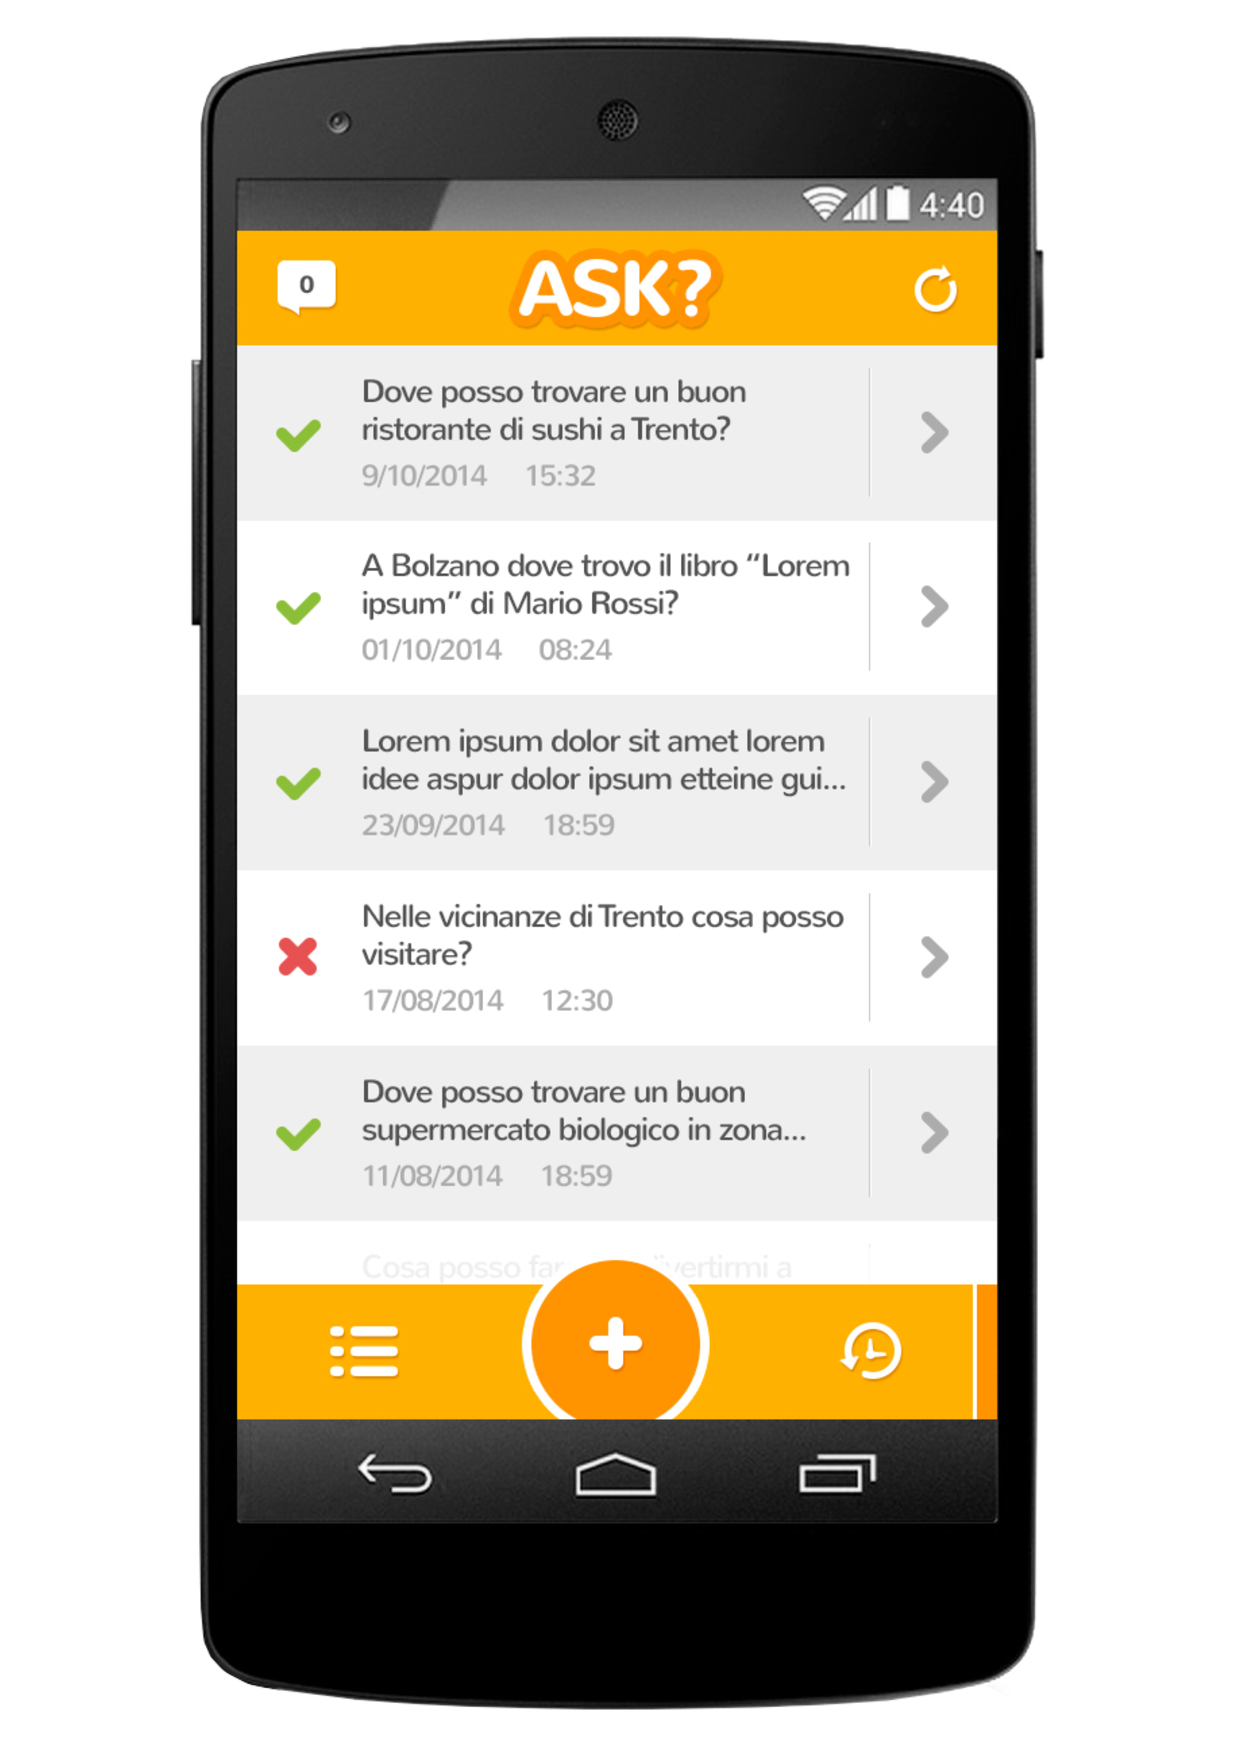
\includegraphics[width=0.2\textwidth]{./figs/ask/ask3.pdf}
    }
    	\subfloat[Answer details\label{subfig-5:dummy}]{%
      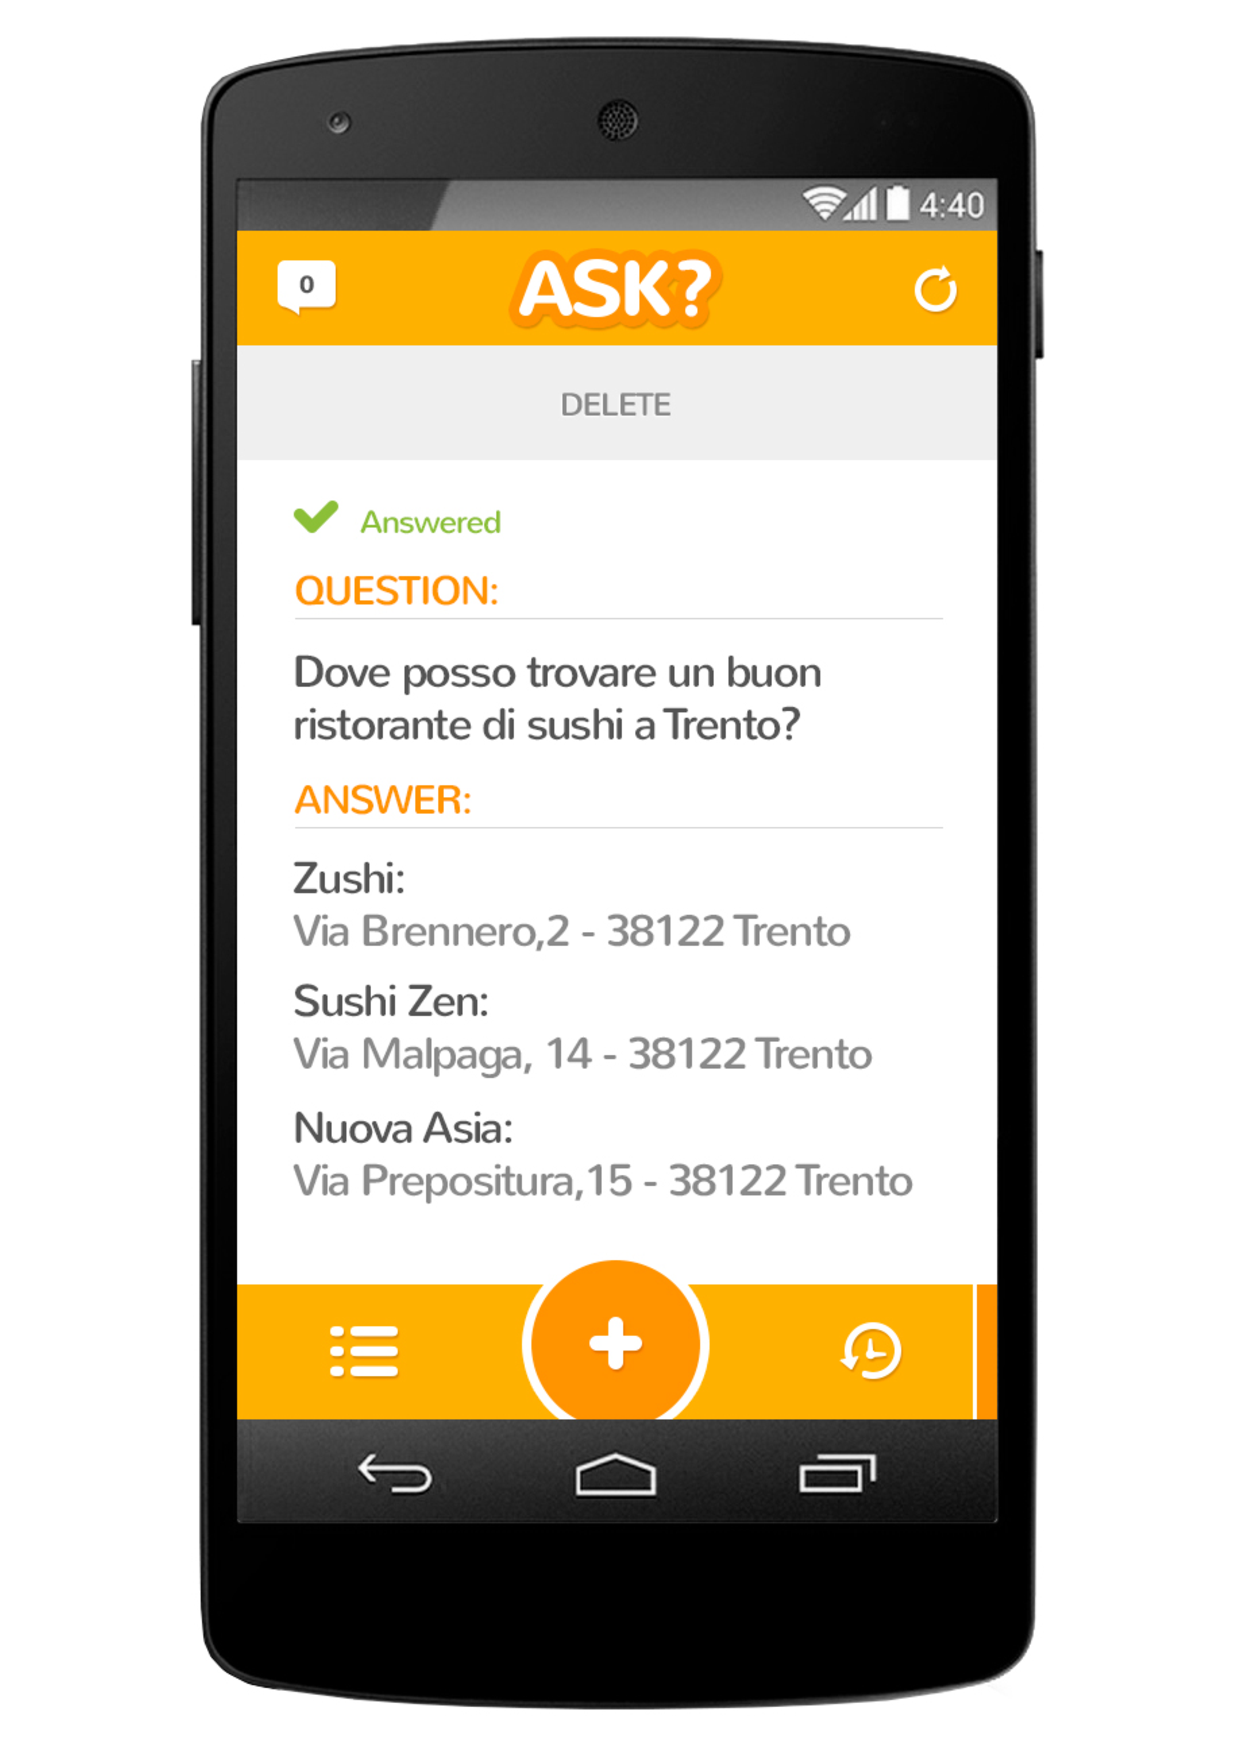
\includegraphics[width=0.2\textwidth]{./figs/ask/ask4.pdf}
    }
    \caption{Ask SmartSociety UX design}
    \label{fig:askpeer}
\end{figure}


\subsection{Example: SmartShare}
\textit{SmartShare} is a ridesharing application in which travellers share a vehicle for a trip and split travel costs such as gas, toll, and parking fees with others that have similar itineraries and time schedules. 
SmartShare reflects important features of HDA-CAS. First, it is a hybrid system, featuring humans who negotiate and perform physical rides as well as machines (intelligent software agents) that recommend routes, match people and monitor rides. SmartShare supports diversity awareness, in terms of users with different preference and affordances as well as different local cultures and values. SmarthShare supports collectives, in terms of both different types of using forming different communities as well as creating geographical clusters of activity. 
%They are diverse, supporting participants who are distributed geographically, come from different backgrounds and have different roles (e.g., driver, passenger). Participants have different travel requirements and preferences and access to different types of information. These aspects interact. For example, while large numbers of participants create more opportunities for participants, they also make it more difficult to allocate rides in an efficient, timely way.
 
%Given these qualities, SmartShare is a perfect setting within which to engage in SmartSociety research as it allows us to study key research questions addressed by the project.

The SmartShare sequence diagram is depicted in Fig.~\ref{fig:smartshare}. Users can post, by using the appropriate app interface, a ride request or ride offer. This includes information on the date, time and destination, as well a set of user preferences (e.g., 'I do not want a driver who smokes in the car') . This request is taken over by the orchestration manager. Constraints matching takes place within the OM, which creates a (plurality of) composition(s), in terms of peers matching constraints, and therefore constituting a potential ride. In the process of finding viable matches, the OM uses the search functionality exposed by the PM. 
%This information, together with the profile of the requesting user, are used by the SmartShare application to create a composition: peers matching both request constraints and user profile are identified and returned as a possible composition. 
The application then goes, using the OM functionality, through the recruitment (negotiation) process, in which each peer identified in the composition is contacted over the preferred communication channel and asked to confirm the participation in the ride. Peers provide individual ride agreement. If all intended peers provide a confirmation, the ride is fully agreed and execution can start. Execution can involve a number of steps, whose transitions are managed by the Execution Manager. Each step may include feedback from the users/peers. 
% Once the negotiation is successfully completed, an agreed ride plan is created, and the task execution (i.e., the actual ride) can take place. 
%This will happen asynchronously with respect to the initial request, on the date and time for which the ride share was searched. Once the ride share is executed the task is concluded.  

\begin{sidewaysfigure}
%\begin{figure}
\centering
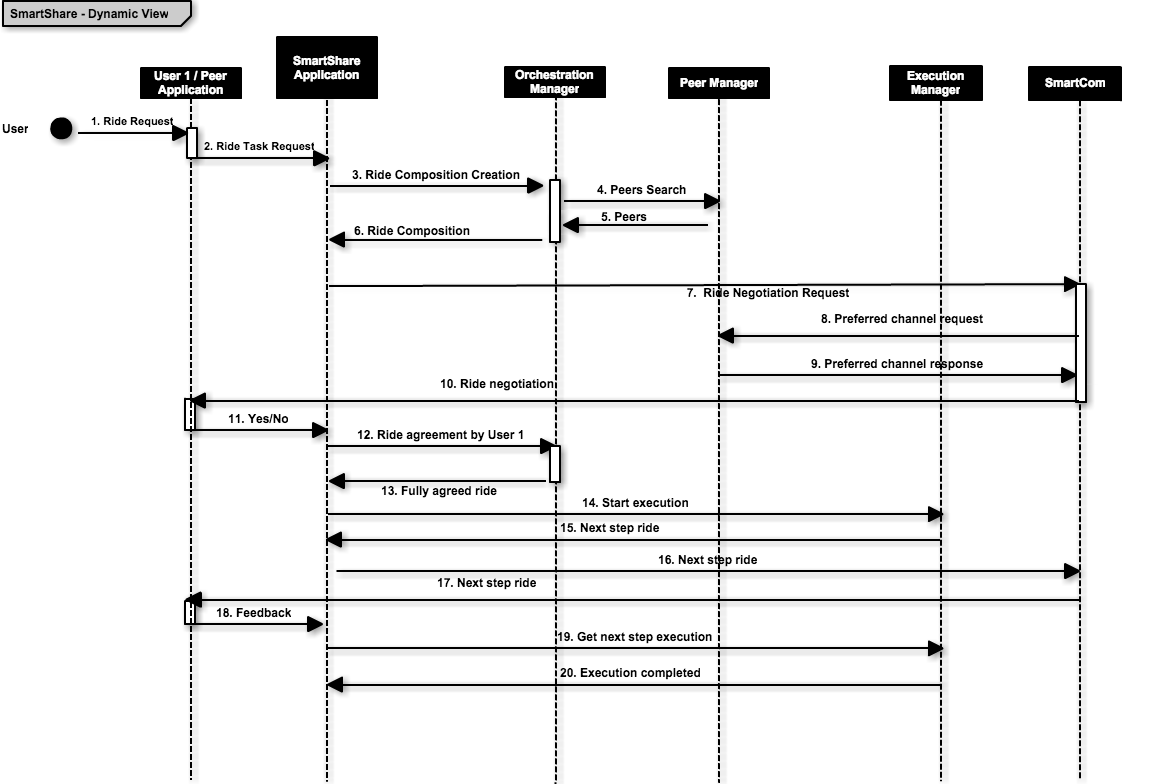
\includegraphics[width=0.9\textwidth]{./figs/sequenceRide}
\caption{Sequence diagram for SmartShare.}
\label{fig:smartshare}
\end{sidewaysfigure}
